\documentclass[]{beamer}
\usepackage[utf8]{inputenc}
\usepackage[T1]{fontenc}
\usepackage{carlito}
\usetheme[horizontal=true, hr=false, pagenumbers=true]{NewPwr}
\usepackage{bibentry}
\usepackage{minted}
\setminted{fontsize=\small,baselinestretch=1}
\usepackage{multicol}
\usepackage{polski}
\usepackage{setspace}

% Build-specific command
\nonstopmode

\onehalfspacing
% \doublespacing

%Information to be included in the title page:
\title{Przewidywanie zapotrzebowania na energię na podstawie danych \textit{PJM Interconnection LLC}}
\subtitle{Przedmiot Monograficzny -- projekt}
\author{Mateusz Bączek, Michał Rajkowski, Konrad Bratek}
\institute{Politechnika Wrocławska}
\date{2023}

\begin{document}

\frame{\titlepage}

\section{Wstęp teoretyczny}

\begin{frame}
\frametitle{Zbiór danych -- PJM Interconnection LLC}
  \begin{figure}
    \centering
    
\includegraphics[width=0.3\linewidth]{pjm-logo.png}
    \vspace{-0.3cm}
    \caption{Logo \textit{PJM interconnection}}
  \end{figure}
  \vspace{-0.5cm}
  \begin{figure}
    \centering
    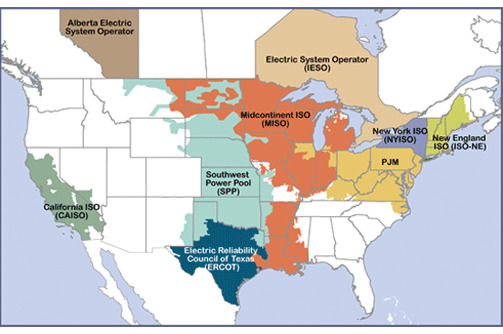
\includegraphics[width=0.6\linewidth]{rto_map.jpg}
    \vspace{-0.3cm}
    \caption{Operatorzy sieci elektrycznej na terenie Stanów Zjednoczonych.}
  \end{figure}

\end{frame}

\begin{frame}
\frametitle{Raport z postępów -- wykonane zadania}

  \begin{enumerate}
    \item Weryfikacja spójności zbioru danych:
      \begin{itemize}
        \item ciągłość danych,
        \item występowanie anomalii,
        \item puste (\textit{null}) wartości,
      \end{itemize}
    \item wyliczenie rozkładów normalnych dla danych:
      \begin{itemize}
        \item weryfikacja czy dane dopasowują się do rozkładu normalnego,
        \item sprawdzenie skośności danych,
      \end{itemize}
  \end{enumerate}

\end{frame}


\begin{frame}
  \frametitle{Przegląd danych}

  \begin{figure}
    \centering
    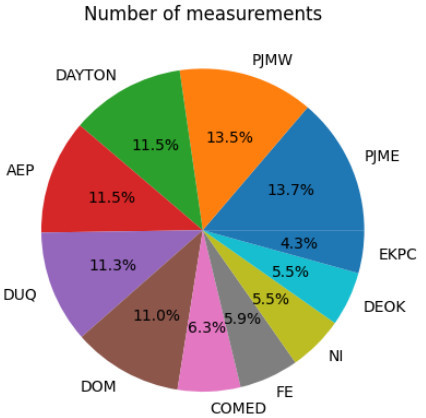
\includegraphics[width=0.5\linewidth]{pie_chart.jpg}
    % \vspace{-0.3cm}
    \caption{Podział liczby pomiarów ze względu na dostawcę.}
  \end{figure}

\end{frame}




\begin{frame}
  \frametitle{Ciągłość danych}

  \begin{figure}
    \centering
    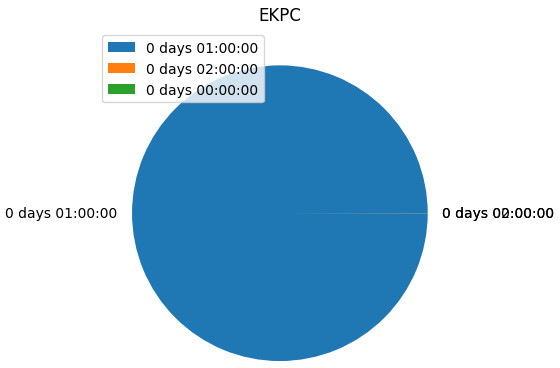
\includegraphics[width=0.6\linewidth]{consistency.jpg}
    % \vspace{-0.3cm}
    \caption{Częstotliwość pomiarów jest spójna w przeważającej większości datasetu.}
  \end{figure}

\end{frame}


\begin{frame}
  \frametitle{Rozkład danych}

  \begin{figure}
    \centering
    \begin{multicols}{2}
      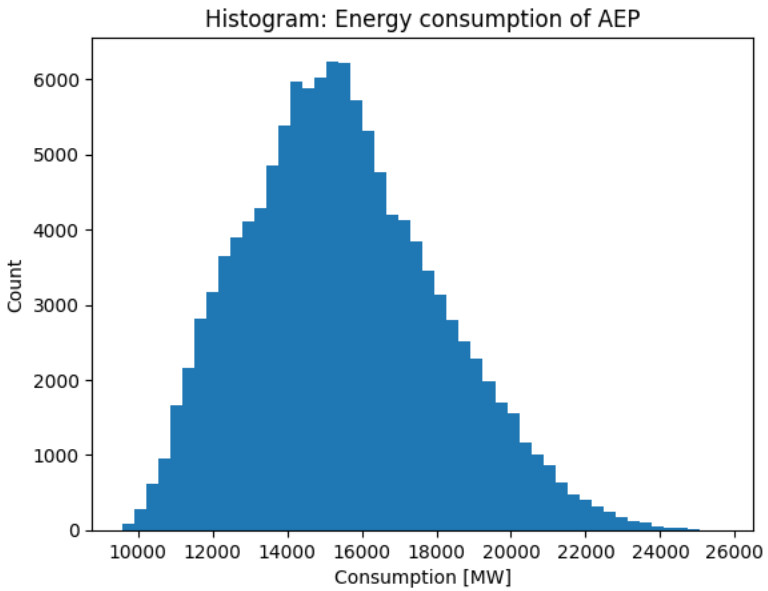
\includegraphics[width=1.0\linewidth]{histogram_1.jpg}
      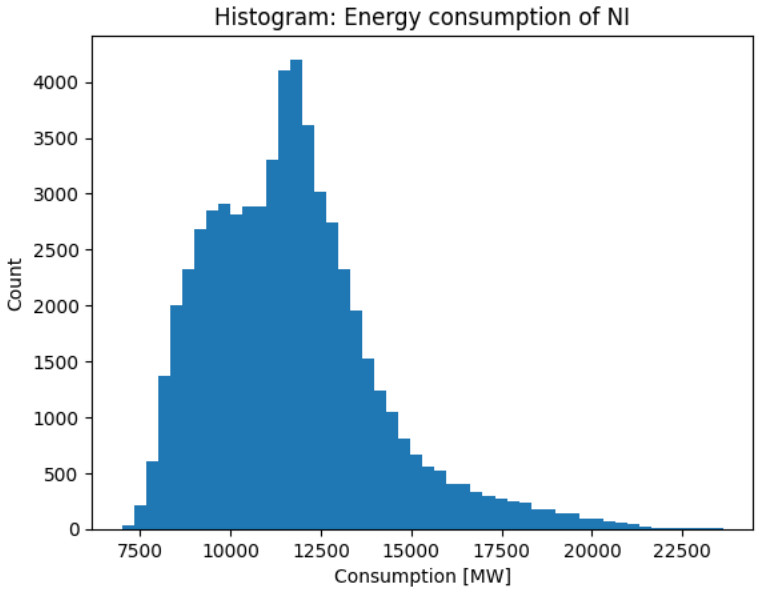
\includegraphics[width=1.0\linewidth]{histogram_2.jpg}
    \end{multicols}
    % \vspace{-0.3cm}
    \caption{
      Zużycie energii ma rozkład ujemno skośny we wszystkich zbiorach.
    }
  \end{figure}

\end{frame}


% \begin{enumerate}
%   \item Przewidywanie zużycia energii na dzień do przodu,
%   \item testy przewidywania w dłuższej perspektywie czasowej (kilka dni/tydzień),
%   \item sprawdzenie trendów zużycia energii podczas świąt, wakacji, itd.
%   \item przetestowanie skuteczności różnych modeli predykcyjnych,
%   \item przetestowanie sprawności modelu na danych od innego dostawcy energetycznego (jeśli uda się znaleźć).
% \end{enumerate}
% \end{frame}

% \section{Bibliografia}

\begin{frame}
  \centering
  \huge{
    Dziękujemy za uwagę!}
\end{frame}


\end{document}

